\documentclass[conference]{IEEEtran}
\IEEEoverridecommandlockouts
% The preceding line is only needed to identify funding in the first footnote. If that is unneeded, please comment it out.
\usepackage{cite}
\usepackage{amsmath,amssymb,amsfonts}
\usepackage{algorithmic}
\usepackage{graphicx}
\usepackage{textcomp}
\usepackage{xcolor}
\usepackage{array}
\def\BibTeX{{\rm B\kern-.05em{\sc i\kern-.025em b}\kern-.08em
    T\kern-.1667em\lower.7ex\hbox{E}\kern-.125emX}}
\begin{document}

\title{{Secure Privacy Preserving Deep Learning against GAN attacks}\\
\author{\IEEEauthorblockN{Aseem Prashar}
\IEEEauthorblockA{\textit{EECS department} \\
\textit{Wichita State University}\\
Wichita, USA \\
prasharaseem@gmail.com}
\and
\IEEEauthorblockN{Sergio Salinas}
\IEEEauthorblockA{\textit{EECS department} \\
\textit{Wichita State University}\\
Wichita, USA \\
sergio.salinasmonroy@wichita.edu}
}
}
\maketitle

\begin{abstract}

Deep learning is a class of machine learning algorithms that use a cascade of multiple layers of nonlinear processing units for feature
extraction and transformation. Each successive layer uses the output from the previous layer as input. Artificial neural network based
deep learning is becoming increasingly popular in classification fields. Deep learning benefits from larger input data sets and can be
revolutionary to organizations that have access to sizable raw data. In
the recent years,  researchers have proposed decentralized collaborative learning architectures that allow multiple participants
multiple participants to share their data to train deep learning models. However, privacy and confidentiality concerns limit the
application of this approach, preventing certain organizations such as medical institutions to fully benefit from collaborative deep
learning. 
%Generative adversarial networks (GANs) consists of two neural
%networks, pitted against one another. They are adept at mimicking any distribution of data and are used widely in image, video and
%voice generation. There has been a recent interest in utilizing the mimicking properties of GANs to fashion attacks on privacy
%preserving deep learning systems. In this attack, GANs are leveraged to generate prototypical samples of the targeted training set that
%was meant to be private. Since the attacks are designed to exploit intrinsic weaknesses in privacy preserving deep learning models,
%they are effective even when differential privacy and obfuscation techniques are employed.
In this paper, we propose a collaborative deep learning approach that allows an organization to collaborate with other entities
to improve its deep-learning model while preserving its privacy. 
%enables a main benefactor to render himself immune to the threats
%posed by a GAN
%based attack. 
Specifically, our proposed system protects the organization's privacy by ...
\end{abstract}

\begin{IEEEkeywords}
Neural Network, Deep learning, GANs
\end{IEEEkeywords}

%---------------------------------------------------------------------------------
\section{Introduction}
%---------------------------------------------------------------------------------
\_To Do\_ : Description of 1- Deep Learning , Neural Network, GAN,

%-----insert my article

%---------------------------------------------------------------------------------
\section{Related Work}
%---------------------------------------------------------------------------------

In the past years neural networks have found application in a wide array of fields.
Deep neural networks have had a significant impact in diverse areas such as video processing \cite{taigman2014deepface}, gaming \cite{chang2016google, lai2015giraffe} and even diagnosis and classification of diseases \cite{cruz2013deep,fakoor2013using}.

Deep learning has outperformed dogmatic techniques in facial detection and image classification\cite{krizhevsky2012imagenet,simard2003best}. Research in speech recognition \cite{hinton2012deep, graves2013speech } indicates that deep learning is on track to even outperform humans.

However areas such as the medical and financial fields that stand to benefit from deep networks also rely heavily on availability of large datasets for training \cite{chicurel2000databasing}. This has however raised some privacy issues.

To combat data privacy concerns some research have explored secure multiparty computations (SMC) as a solution.

In \cite{vaidya2003leveraging}, the researchers survey secure multi-party computation and provide a method to an efficient protocol where a three party system can be used to construct an efficient peer-to-peer secure multi-party protocol.

In \cite{7040943}, the authors survey multi party computation as well as other techniques. They also evaluate SMC's effectiveness and cost in context of secure data processing.

SMC's application in secure computation of private data is explored in \cite{sheikh2010distributed}. The authors propose a novel protocol that divides and distributes private data blocks among participants. This facilitates a scenario in which semi honest parties are incapable of discovering private data of other parties. This technique is however contingent on the malicious parties being semi-honest parties.

In \cite{miyajima2016new}, the authors propose to solve security risks associated with cloud computing using SMC. They propose a back propagation learning method for secure data computation and learning on cloud based system. The authors acknowledge that this technique can be computationally expensive for the clients participating in the system.

To overcome constraints in a mobile user setting, some researchers have proposed a protocol to aggregate user data by leveraging SMC \cite{bonawitz2017practical}. They focus their work on creating a robust protocol that maintains its efficacy even if there are client dropouts. 

Some research has also been done in the field of differential privacy to guarantee data privacy protection.
In \cite{abadi2016deep}, the authors analyze the privacy cost, complexity and training efficiency of neural networks with differential privacy. They propose a novel algorithmic technique for training neural network with a modest privacy costs with a viable software complexity. Their work however does not account for distributive collaborative deep learning. Since differential privacy is hinged on adding nose to the data, the added noise will scale with size of the participants. Ultimately, the amount of noise added will render the shared data to have no practical use.

In \cite {song2013stochastic}, the authors investigate effects of differential privacy on mini batch SGD. They document their observation that increased batch size improves can help ameliorate the impact of differential privacy on the variability of SGD. The authors, however, also observe an upper limit to the batch that can be utilized to control the variability produced by the privacy preserving noise.
   
The authors in \cite{chase2017private} propose a protocol that merges SMC as well differential privacy for learning neural networks in a collaborative way. Since differential privacy is does not scale and SMC does not guarantee the privacy of the end result, the authors attempt the bridge the two to architect a stronger protocol.
However, their solution also rests on the assumption of semi honest parties and does not account of malicious participants at all. The authors also observe that accuracies generated by their protocol drop with increasing parameters in the network. This prevents the propose protocol from being scalable.

In \cite{shokri2015privacy} the authors propose a system that enables collaborative training for neural networks in a privacy preserving manner. In the paper the authors design and test a protocol in which the participants share a small subset of parameters from their trained neural networks. These parameters are then aggregated on independent server. This enables the participants to preserve the privacy of their dataset while drawing benefits from other participants trained model.

In \cite{hitaj2017deep}, the authors outline a possible attack that exploits the architectural weaknesses in the collaborative learning system proposed in \cite{abadi2016deep}. The attack proposed in \cite{hitaj2017deep} leverages Generative adversarial networks as a malicious participant and is therefore immune to majority of obfuscation techniques. The authors claim that the  deceptive adversarial influence aspect of their attack is arguably a more potent threat than the ones posed by techniques involving Model Inversion attacks in \cite{deng2012mnist}.

%---------------------------------------------------------------------------------
\section{Background on Deep Neural Networks}
%---------------------------------------------------------------------------------
Deep Learning  is a subset of machine learning that excels at extracting complex information from high dimensional data. Unlike traditional machine learning deep learning workflow does not involve manual feature extraction. It is essentially an end-to-end process where the network can be trained on raw data without the burden of preprocessing it.
Deep Learning also scales with the data size, producing more accurate results with larger datasets.
These advantages make Deep learning a very effective technique to perform classification tasks.

Deep learning architectures are comprised of several neural networks organized in layers. Neural networks consist of 3 types of layers. Input layers are first layers that receive input, ouput layer is the last layer in the network. All layer between input and output layer are hidden layers. Traditionally, Deep networks contain 2 or more hidden layers. These multiple layers enable Deep networks to compute nonlinear functions of abstract data features.
One of the basic Deep learning neural network architecture is the multilayer perception (MLP). It is a feed-forward based network implying it has no feedback loops and instead directly maps inputs onto a set of outputs. 

MLP architecture is composed of multiple layers where each layer consists of many inter-connected nodes. The layers are fully connected to the previous as well as the next layer in the architecture. The output of a single node within the layer is a function of the weighted average of the inputs connected to the node from the previous layers. In a typical network, each neuron also receives an additional input from a special neuron called the bias.  Together, the weights and biases of neural network are called its parameters. The weighted average of inputs plus the bias is referred to as the total input for the neuron. The final output of the neuron is computed by applying a activation function to the computed total input. This activation function is crucial in introducing non-linearity in neural networks. The non-linearity allows the modelling of complex data that linear regression models lack the dimensionality to do.
Formally, the output of neuron at layer $k$ is defined as follows:
$$a_k=f(W_k a_{k-1})$$
Where $f$ is the activation function.  $W_k$ is the weight matrix of at layer $k$ which controls how input signal from previous layer, $a_{k-1}$ affects the output of the current neuron. 
There are several non-linear activation functions that can be used such as sigmoid function which outputs values between 0 and 1, normalizing the output of each neuron. Hyperbolic tangent activation function is zero centered and makes it easier to model inputs that have strongly negative, neutral or positive values. Rectified Linear Unit (ReLU) is an increasing popular activation function that aids in the quick convergence of the network. In a network that is tasked to classify inputs to one of the $j$ fixed number of outputs, the output layer typically deploys SoftMax activation function, given by 
$f(z_j) = e^{zj}\cdot (\sum_ke^{zk})^-1, \forall j$.
This function normalizes the output for each class between 0 and 1 and divides it by their sum, resulting in a probability score that the given input belongs to class $j$. 
Figure \ref{fig:SimplNN} shows the structure of a typical classification deep neural network with $m$ inputs mapped to $j$ ouputs. The neural network has $N$ hidden layers and each layer has $I$ neurons.
\begin{figure}[!h]
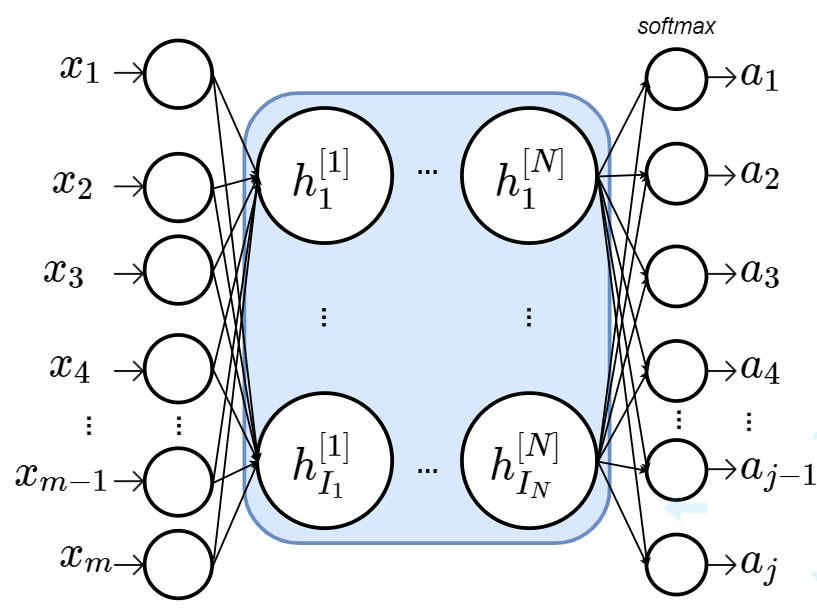
\includegraphics[width=8cm, keepaspectratio]{SimpleNN}
\caption{Simple neural network depicting $m$ inputs, $j$ outputs  $N$  hidden layers and with $I$ neuron in layer.}
\label{fig:SimplNN}

\end{figure}



%For professor: Should i insert activation function formula for each of the mentioned functions?

Before a neural network can be deployed, it needs to be trained to model non-linear high dimensional functions. The training of a neural network involves selecting the exact set of parameters, weights, biases and activation function that meet its specified objective. There are several algorithms that can tackle this non-linear optimization problem. A training dataset is a dataset of sample inputs which has  known outputs or labels. In supervised learning,  we feed the inputs from a training dataset to the neural network during its training phase and compare computed output with the corresponding labels.

Some of the most popular algorithms deployed in the training phase are variants of gradient descent (GD)  algorithm. In simple terms, the GD algorithm calculates the derivative of the function being optimized with respect to each of the current parameters. It then updates the parameters and repeats the process iteratively to achieve more accuracy. 
Gradients in Deep network are computed after both the feed forward and back propagation steps. In forward propagation, the inputs from a training set are passed to the network and its output is recorded. We then compare the computed output and provided labels to calculate the error or loss function. The error function is given by the difference between the label of the training set and the computed output by the neural network. The backpropagation algorithm then finds the partial derivative of the error function with respect to each neuron. This highlights how each neuron has contributed to the total error. We then use each neuron's computed error contribution and its corresponding activation value to calculate gradient. The parameters in the network are then adjusted to reduce the computed gradient.
 repeat these steps of forward pass, error calculation, back propagation and parameter update iteratively until the desired objective function is achieved.



%---------------------------------------------------------------------------------
\section{Background on Stochastic Gradient Descent}
%--------------------------------------------------------------------------------- 
Gradient Descent (GD) is an iterative algorithm that is often used to calculate the parameters of neural
networks, i.e., their weights and biases. At each iteration, the  algorithm updates the parameters based on the gradient of the 
an error function evaluated with the current parameters. The iterations continue until a minimum of  is reached. Since the objective
function is non-linear, the algorithm can only guarantee that it converges to a local minimum.

The GD algorithm works to minimize the error function by taking 'steps' towards the desired minimum. A learning rate, $\alpha$ is chosen which dictates the size of each step at every iteration.
Selecting an optimal learning rate is crucial since a smaller learning rate results in many steps to reach the minima. This causes longer and computationally expensive convergence time.
On the other hand, if the chosen learning rate is too large the algorithm can fail to converge and overshoot the desired minimum. 
Optimal learning rates are generally chosen through trial and error . Some of the most commonly used learning rates are 0.001, 0.003 and 0.01
We then pass all of our data through the network and calculate the error function. Typically, the error function is the average of the sums of the difference between the predicted value and the given label. Fornally we can define the mean squared error function, E as follows:
$$ E= \frac{1}{n} \sum_{n=1}^{n}(y_i -\hat{y_i}),$$
where $n$ is the the size of the dataset, $y_i$ is the output calculated by the neural network and $\hat{y_i}$ is the actual label for the sample $i$.

In the next part of GD algorithm we back-propagate this error. This is done by computing the partial derivative of the error function with respect to each parameter in the current configuration of the network. This value is referred to as the gradient. We obtain the new value of parameters by subtracting the product of learning rate and gradient of each parameter from each original parameter. 
Consider E to be the error function over the entire dataset, then the new value of parameter $w_i$ is given by:

%\begin{equation*}
 $$w_j = w_j -\alpha \frac{\partial E}{\partial w_j} $$
%\end{equation*}

This process is iteratively repeated until the cost function converges and we minimize the error.

Although GD is effective at finding the parameters of DNNs, all  training samples in the dataset need to be processed before a single updates is made ot the parameters. That is,  to take a single step towards minimizing the error function, the algorithm processes all the input samples. This is computationally intensive and time consuming. To overcome this challenge, Stochastic Gradient Descent(SGD) has been
proposed. Unlike GD where all samples in the data set are used in a single iteration, SGD only selects a random subset
of samples for calculating the gradient and updating the parameters at each iteration. SGD then uses this fraction of dataset do a forward pass, calculate error and back propagate the to find the gradients of each parameter. This process is identical to the one outlined for GS. 
However, Since SGD only uses a fraction of the training
data set during each iteration, its computing time is significantly smaller compared to GD. If the fraction of dataset is a single sample, then the algorithm is said to maximum stochasticity. If the fraction is significantly smaller than the size of the total dataset available and greater than one, then SGD is also referred to as Mini-batch Gradient Descent.

Since SGD explores different parts of the solution space by randomly selecting samples at each iteration, it has a higher probability of escaping local minima. However, the randomized selection of data samples can also cause updates made to the parameters to be less accurate. This results in an overall meandering path to the local minima. 

To choose the right algorithm for optimization, one can choose between speed (provided by SGD) and accuracy of each step (provided by GD). For larger datasets SGD and Mini-Batch GD is preferred since the taking multiple slightly inaccurate updates is preferable over a single slower update in one epoch.
The size of the subset of samples, called mini-batch, used at each iteration has to be chosen carefully. A small batch can reduce the
computing time at each iteration, but may increase the number of iterations needed to converge. 


Formally, the SGD can is defined as follows. 
Let $w$ denote the flattened
vector of all weights and biases of a deep neural
network. Let $E$ be an error function which is defined as the difference between the actual output of the objective function and the
predicted output of the network. 
%Our aim is to compute the slope of the cost function and the direction we should move to update our
%parameters. 
Then the $j$th parameter of $w$ is give by:
%\begin{equation*}
\begin{align}\label{eq:SGD}
w_j = w_j -\alpha \frac{\partial E_i}{\partial w_j}, 
\end{align}
where $\alpha$ is the learning rate,  $E_i$ is the value of the error function computed over minibatch $i$, and  
$\frac{\partial E_i}{\partial w_j}$ denotes the partial derivative of $E_i$ and $w_j$. 
 

%---------------------------------------------------------------------------------
\section{Problem Formulation}
%---------------------------------------------------------------------------------
In this section, we describe our considered collaborative deep learning model, and the threat model. 

%---------------------------------------------------------------------------------
\subsection{System Model} \label{sec:systemModel}
%---------------------------------------------------------------------------------

In this section, we describe a deep learning system with a set of users $\mathcal{U}= \{u_0, \dots,u_N\}$, where $N$ is the total
number of
users. Each user has a collection of
private dataset  $\mathcal{D}= \{d_0, \dots,d_N\}$. 
%We assume a reference  participant, $u_0$ whose dataset $d_0$ is significantly smaller
%than datasets $d_1$ to $d_N$ belonging to users $u_o$ to $u_N$. 
Let $w_i$ be the flattened vector of parameters for the $i$th user. The
deep learning system aims to share parameters of each user $u_0$ to $u_N$  trained privately on datasets $d_0$ to $d_N$ in a privacy
preserving manner.

To do this, all participants in this system agree in advance on a
common network architecture and common learning objective. The system also includes a secure parameter server (PS), which maintains the
latest values of parameters uploaded given by $w^{(global)}$. Each user, $u_i$ in the system selects a $\theta_d^{i}$, which is the fraction of  $w^{(global)}$ parameters that the user will download from the PS. 
The user $u_i$ also choses a value $\theta_u^{i}$ which is the fraction of $w_i$ that user chooses to upload to the PS.

Each participant, $u_i$ randomly initializes its parameters $w_i$ and selects a learning rate, $\alpha$.
The participant then downloads $|\theta_d^{i} \times w_i|$ parameters from PS and overwrites its corresponding local parameters.
$u_i$ then runs the stochastic gradient descent algorithm for one epoch on its local dataset and trains its model. The local parameter vector, $w_i$ is updated according to \eqref{eq:SGD}. The SGD yields a new set of parameters, $w_i^{(new)}$.
In the next step, $u_i$ computes the parameter gradient $\Delta w_i$ which is vector of changes in all local parameters due to the SGD. This is computed by
$$\Delta w_i =  w_i^{(new)} -  w_i$$ 
The gradient  $\Delta w_i$ is indicative of how much each parameter has to change to more accurately perform regression on the local dataset $d_i$.
Consider $S$ to be a set of indices with the top  $|\theta_u^{i} \times \Delta w_i|$ values in $\Delta w_i$ 
The participant then uploads  $\Delta w_S$ values to the PS.
These uploaded values represent the parameters in the local model that have undergone the largest changes due to the SGD. 

When a participants makes a valid attempt to upload $\Delta w_S$ parameters to the PS, parameter vector of PS,  $w^{(global)}$, is updated as follows:
$$w^{(global)} =  w^{(global)} +  \Delta w_S$$

In this scenario we assume all participants, $u_0$ to $u_N$, interact with the server atomically.
That is, at any given time, only one participant can upload or download parameters from the server. This prevents over writing of parameters or race conditions from occurring within the server.

%--------------------------------------------------------------------------------------------
\section{Neural Network Architecture}
%--------------------------------------------------------------------------------------------

In this paper we use a multilayer perceptron (MLP) in a classic feed forward arrangement. Each layer in the network is fully connected to the next layer. The networks takes images as its input to its first layer. It then funnels this input through multiple hidden layers. An activation function is then applied to the output of each hidden layer. For this network we choose the Rectified Linear Unit or ReLU as the activation function. Since this network serves as a classification network, the log soft max activation function is applied to the last layer. This results in outputs that are squashed into probabilities that sum to one. 
Figure \ref{fig:ClassNN} shows the structure of a typical feed forward MLP deep neural network. The network is fed a raw image of  $m \times m$ pixels. Each pixel is an individual input which is funneled through $N$ hidden layers and ReLU activation function with $I$ neurons in each layer. The neural network produces $j$ outpputs with each putput mapping to a single class. In a classification network such as this, each output $a_1$ through $a_j$ reflects the probability of the image belonging to that class. All ouputs pass throught the softmax layer and therefore sum to 1. 

\begin{figure}[!h]
\includegraphics[width=8cm, keepaspectratio]{ClassificationNN}
\caption{Neural network depicting an image with $m \times m$ pixels fed as input, $j$ outputs  $N$  hidden layers and with $I$ neurons in layer.}
\label{fig:ClassNN}
\end{figure}
The parameter server is responsible for maintaining the current values of all parameters. Since it should be accessible to all
participants , the server can be implemented as any form of updatable cloud storage. However, for the purpose of this experiment we
chose to implement it as another neural network. 




%---------------------------------------------------------------------------------
\subsection{Threat Model}
%---------------------------------------------------------------------------------
The core prinicple motivating distributed learning is the idea that users do not wish to share their private training data. This data can be sensitive and an unverified user might attempt to maliciously violate the sharer's privacy on the pretext of model training.

We consider a malicious threat model for the parameter server and the collaborators. Specifically, the collaborators will attempt to learn private information about the reference user's dataset based on the parameters that the reference user uploads. 
In addition, one or multiple  collaborators will attempt to actively trick the reference user to reveal its private information by uploading malicious parameters. 

Instead of sharing the parameters of its deep neural, the malicious party will collect the parameters from its victim user. The malicious party will then replicate the victim's data, ultimately violating the the victim's privacy.
  
Since the threat is not dependent on the adversary compromising the
central Parameter Server, it remains viable. In effect, the adversary does not have to control the PS or the service
provider to execute his attack. The attack is more effective when adversarial influence is exercised \cite{hitaj2017deep}. This would imply that the adversary is an active participant that is adapting his gradients in real time during the current learning process.

%describe an attack that results in privacy leakage in
%collaborative deep learning system proposed in
%\cite{Shokri}.  The attack results in a malicious user inferring sensitive information from a victim's dataset. 

%Specifically, the proposed attack the goal of the  adversary is to extract information from a victim about a class of data he does
%not own. The
%adversary deceives victim into releasing more information about the specific class by presenting himself as an honest participant in
%the collaborative learning  process.    The adversary does launches the
%attack by pretending to be an honest participant and building a local GAN unbeknownst to the other participants.

%The threat model is dependent on an active insider. However, 

%\subsection{Attack Posed}

In particular the attack operates as follows. Suppose all participants including the adversary agree on general specifications such as
the type of neural network and labels on which training would take place as described in Section \ref{sec:systemModel}. Let another
participant in the collaborative deep learning
model be the victim $u_V\in\mathcal{U}$ that declares the labels $[a,b]$. The adversary $u_A\in\mathcal{U}$ declares labels $[b,c]$ implying that the
adversary has no data on class $a$. By deploying the attack, the adversary stands to gain useful information about class $a$.

The adversary then uses the private GAN to generate models that look like class $a$, which the adversary deceivingly mislabels as $c$.
This prompts the victim  $u_V$ to release more information about the class $a$ in order to distinguish between classes 
$a$ and $c$. Therefore the victim releases more data on class a now than he initially intended to.

This can be further summarized as follows:
\begin {enumerate}
\item Assuming victim $u_V$ declares labels $[a,b]$ and adversary $u_A$ declares labels $[b,c]$
\item We then run the collaborative learning protocol for several epoch and stop when we reach a specified accuracy.
\item During this process, the $u_V$ downloads a percentage of parameters from parameter Server and updates his local model.
\item $u_V$'s local model is trained on classes $a$ and $b$
\item $u_V$ uploads a section of his model to Parameter Server
\item The adversary trains is slotted to engage with the Parameter Server
\item $u_A$ downloads the percentage of parameters from the PS and updates his model
\item $u_A$ then trains his local GAN to mimic class $a$.
\item $u_A$ generates class a samples from the GAN and mislabels them intentionally as class c.
\item $u_A$ uploads a percentage of his parameters to the PS
\end {enumerate}
During the process of convergence, $u_A$ will be able to covertly exert influence on the learning process via the mislabeling of class
$a$.

In this paper, we present a collaborative learning scenario that prevents the reference user from releasing more
information about a class, and ultimately it protects the reference user's privacy. We design the interaction of the reference user
with Parameter Server such that $u_V$ is not RefU

\section{A Privacy-preserving Collaborative Learning Algorithm}

\begin{figure}[!h]
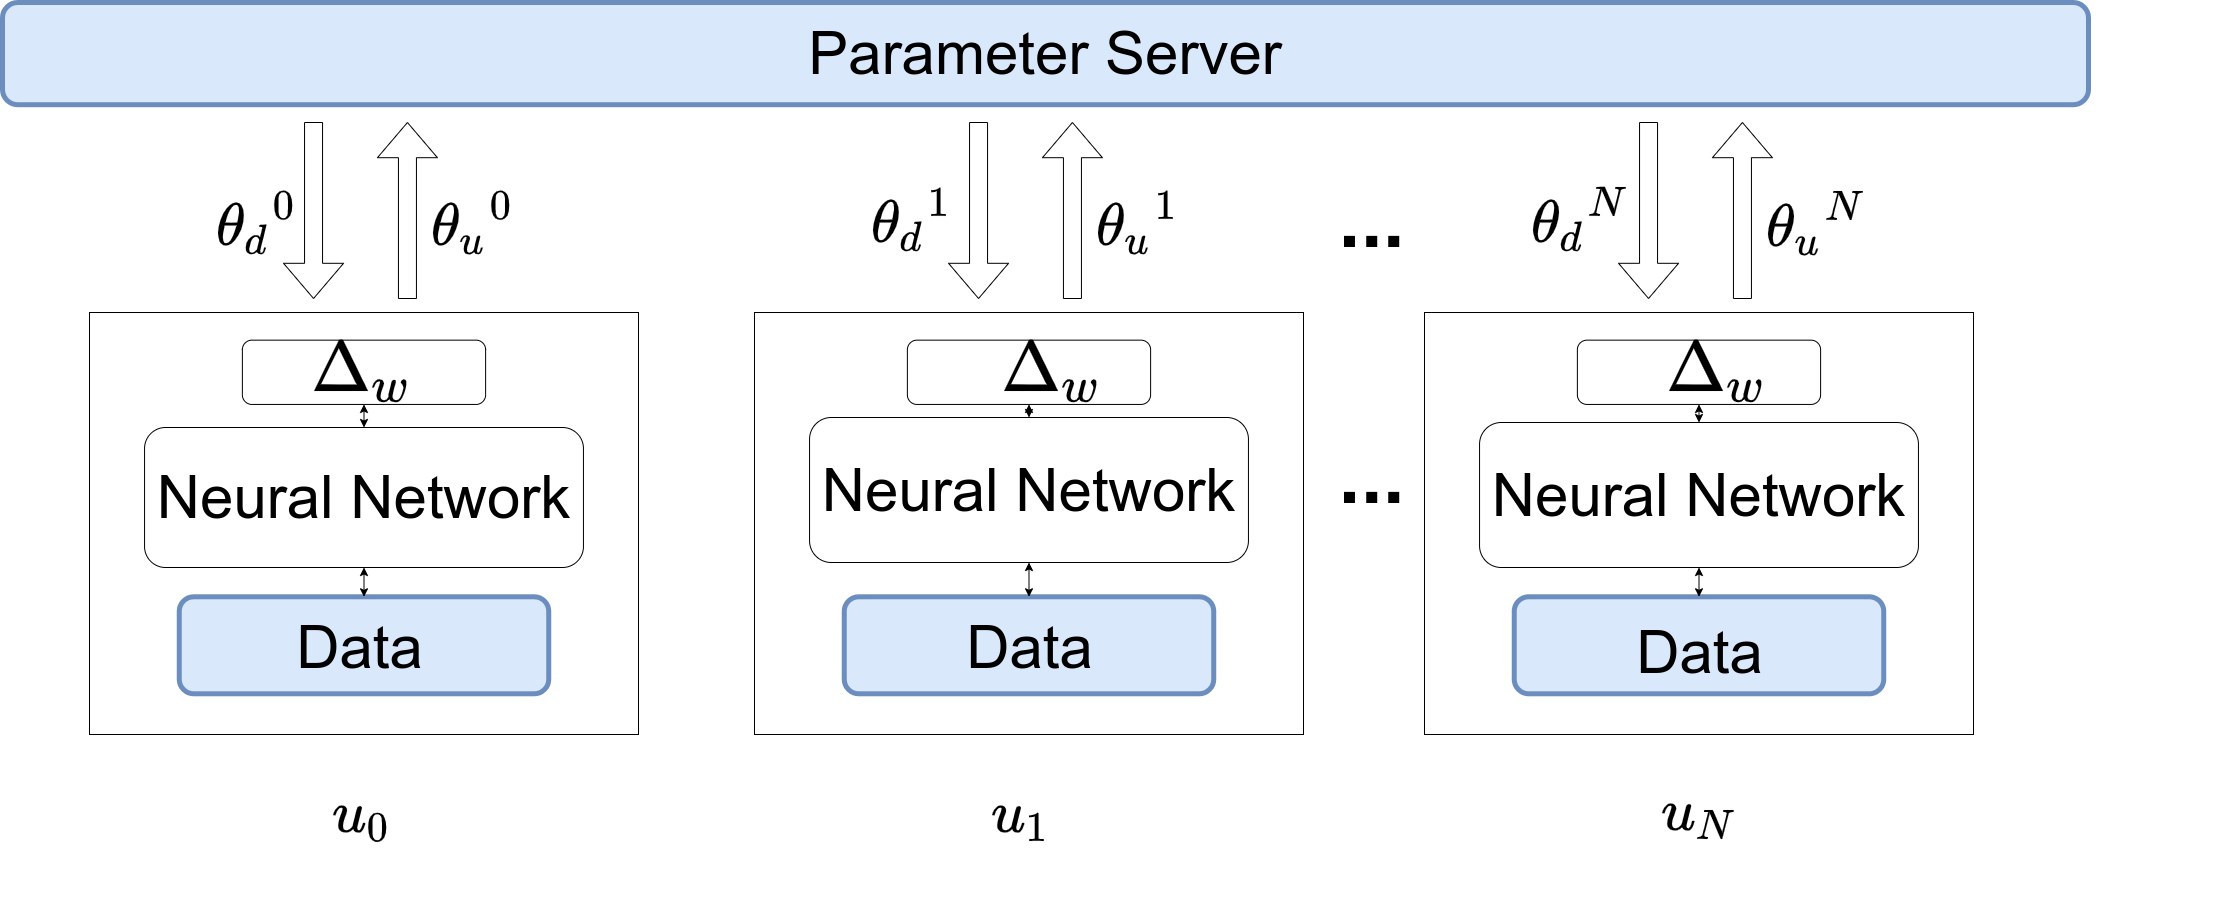
\includegraphics[width=8cm, keepaspectratio]{HighLevelArch}
\caption{High level architecture of our proposed neural network.}
\label{fig:HighLevel}
\end{figure}

This architecture works by ensuring privacy to the reference user by limiting its exposure to other collaborators. We structure this algorithm such that a primary participant, the reference user, $r_0$ benefits the most and is afforded the highest level of protection against GAN-based attacks. We envision this architecture materializing in a manner that involves the reference user compensating other collaborators for the parameters and abstract data to train its model. Since the architecture inherently obscures the absolute data, we are also able to preserves privacy for paid collaborators involved.


Specifically, we propose a system that considers a reference participant with a much smaller data set as the most significant benefactor of this architecture. We consider $u_0\in\mathcal{U}$ to be our reference user with reference dataset $d_0\in\mathcal{D}$ such that $d_0$ is much smaller than all other $d \in\mathcal{D}$


We structure the system to ensure that the privacy of the reference
user, $u_0$ is not affected by the inventive GAN based attack proposed in \cite{hitaj2017deep}. Table \ref{table:1} summarises the notations used in this
paper.

\begin{table}[!h]
\centering
\caption{Table1: Summary of notations used in the paper}
\label{table:1}
\begin{tabular}{ | m{0.12\columnwidth} | m{0.8\columnwidth}| } 
\hline
\textbf{Notation} & \textbf{Description} \\
 \hline\hline

$N$ & Number of participants excpet the system\\
\hline
$u_0$ & Reference User and the  main benefactor of the architecture \\
\hline
$M$ & Mini batch size used for stochastic gradient descent\\
\hline
$\theta_d$, $\theta_u$ & Fraction of parameters selected for download and upload from total available parameters \\
\hline
$W_k$ & Weight matrix for layer K in the neural network\\
\hline
$w$ & Flattened vector of all parameters in the neural network. \\
\hline
$\Delta w$ & Vector of changes in all local parameters due to SGD\\
\hline
$w^{(global)}$ & Flattened parameter vector for server\\
\hline
$E$ & Error Function defining the difference btween the computed value and expected value of the objective function \\
\hline
$\alpha$ & Learning rate of the stochastic gradient descent algorithm\\
\hline
$S$ & Set of $\theta_u$ largest indices selected from $w$ \\
\hline
\end{tabular}
\end{table}


 
We define the following terms, $\theta_u$
$R$
The Algorithm works as follows:
\begin {enumerate}
\item A pool of participants is created where each participant has a sizeable dataset
\item Out of the pool of participants, a random subsection of participants is selected to interact with the PS in this period. We call this period a round which is denoted by $r$.
\item In each round, $r_i$, the selected participant, $u_i$ is able to interact with the PS such that no other participant can interact with the PS at the same time.
\item During its interaction with PS, the participant will perform the following steps:
\begin {enumerate}
  \item train independantly on its local dataset for one epoch, to calculate parameter gradient, $\Delta w$ 
  \item  at the end of the epoch, $u_i$ will select the $\theta_u$ highest gradients, $\Delta w$. The $u_i$ uploads these values to the PS.
  \end {enumerate}
\item For each subsequent epoch, the participant will first download $\theta_d$ percentage of parameters from the server. The participant will then repeat the steps a and b.
\item We repeat these steps for every participant selected in the round. At the end of the round, the reference user downloads $\theta_d$ percentage of parameters from the PS.
\item The reference user then trains its model locally on its small dataset. 

\end {enumerate}
As you can see the, the reference user does not share its parameters with other users. It benefits from random particpants from the architecture but does not expose itself to any attacks. Since the participants selected from the pool each round are randomized, we ..



%-------------------------------------------------------------------------------
\section{Experimental Setup}
%-------------------------------------------------------------------------------

We evaluate the learning performance of the reference user under our proposed privacy-preserving collaborative learning algorithm. We
measure ... and compare it to a the learning performance of a traditional deep neural network without collaborative learning. 
%We wrote the source code based on the pseudocode provided in paper \cite{Shokri}. 
We implement all algorithms using Torch with the neural network packages in the scripting language LUAJIT, and run them on an M4 instance on the Amazon Web Service's Elastic Compute Cloud (AWS EC2).

For this experiment, we implement a similar neural network structure for the reference user as well as other participants. Although one can chose any neural network architecture, we use a multilayer perceptron (MLP) in a classic feed forward arrangement. 
Each neural network is designed to have 1024 inputs
corresponding to each pixel in the provided 32x 32 pixel image of a handwritten number \cite{deng2012mnist}. The output layer is a
tensor of size 10 where each output corresponds to the probability that the given input is a specific number between 0 and 9. The model
also has 2 hidden layers where an activation function is applied to the output of each hidden layer.
Initially, the input is reshaped into a 1 dimensional tensor of size 1024 and funneled to the first hidden layer. The hidden layers are constructed via \textit{nn.Linear()} via which linear transformation can be applied. It then produces a tensor of size 128 as its output. The second hidden layer accepts a tensor of size 128 as input to yield a tensor of size 64 as output. We use a non-linear activation function called Rectified Linear Unit (ReLU) which is applied after each hidden layer. The last layer of the model is a log soft max layer coded by the \textit{nn.LogSoftMax()} module.  This activation function is usually applied to the end of all classification models where it squashes the inputs into probabilities that sum to one.
The Architecture described above are represented in Figure\ref{fig:MLPArch} as printed out by Torch7

%We were able to replicate their original setup using
%Torch and nn packages in LUAJIT scripting language.  
%The tests on the proposed solution were run and hosted 


We used the MLP implementation of neural network using the function \textit{nn.Sequential} container via the Torch nn package. They are
fully connected and the neural network has input data of size 1024 (32 x 32) and feed fowards

%-------------------------------------------------------------------------------
\subsection{Datasets}
%-------------------------------------------------------------------------------
We conducted our experiments using the MNIST dataset \cite{deng2012mnist}. The MNIST dataset is a standard dataset used in image
recognition.
It contains images of hand-written grayscale digits ranging from 0 to 9. The dimension of each image is 32 X 32 pixels. There
are 60,000 such images in their training dataset and 10,000 images in their test dataset.

For this experiment, we normalize the images so that they are centered. 

We set the size of the local dataset of each participant to 1 \% of the training dataset images. 
The Reference User starts with a training set of 60 images.



%--------------------------------------------------------------------------------------------
\subsection{Hyperparameter Setup}

%--------------------------------------------------------------------------------------------
Hyperparameters are parameters that control the collaborative learning process. Unlike the actual neural-network parameters, they are usually set before the training commences and remain unchanged during the process.
They are crucial since they directly influence the behavior of training algorithm and have a large impact on the performance and accuracy o the model.
The learning rate is set at $0.1$ and weight decay is set to $1e-7$. The batch size is 10 samples and the number of participants is 20. We vary the $\theta_u$ and epochs in different scenarios. 

\begin{figure}[!h]
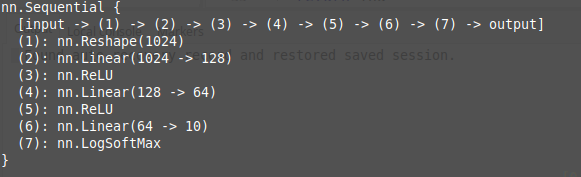
\includegraphics[width=8cm, keepaspectratio]{MLPArchitecture}
\caption{MLP architecture used for MNIST related experiments, as printed ou by Torch}
\label{fig:MLPArch}

\end{figure}


%--------------------------------------------------------------------------------------------
%\subsection{Framework}
%---------------------------------------------------------------------------------------------

%We conduct our experiment within the Torch 7 and Torch 7 nn framework. Torch is a popular framework utilized for deep learning by major
%software companies. The code for the experiment is written in LuaJIT which is a scripting language based on Lua.  We deploy our
%architectural framework with multiple neural networks on the AWS EC-2 machine to leverage greater processing speed.


\section{Experiment Results}

Baseline results: accuracy, training time, training loss, testing loss, plot accuracy under varying number of participants, results

\begin{figure}[!h]
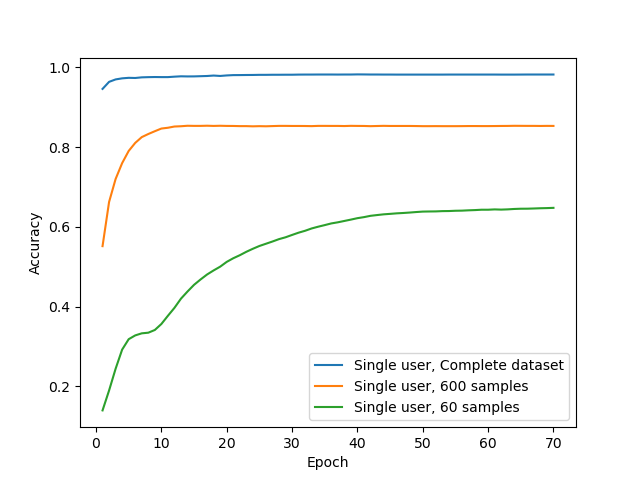
\includegraphics[width=8cm, keepaspectratio]{SingleUserBaselines}
\caption{Single User with varying sample size.}
\label{fig:SingleUser}
\end{figure}

under varying hyperparameters (number of layers, alpha, etc). Matplotlib. Matlab


REsults under your approach: accuracy, training time, training loss, testing loss, plot accuracy under varying number of participants.


\begin{figure}[!h]
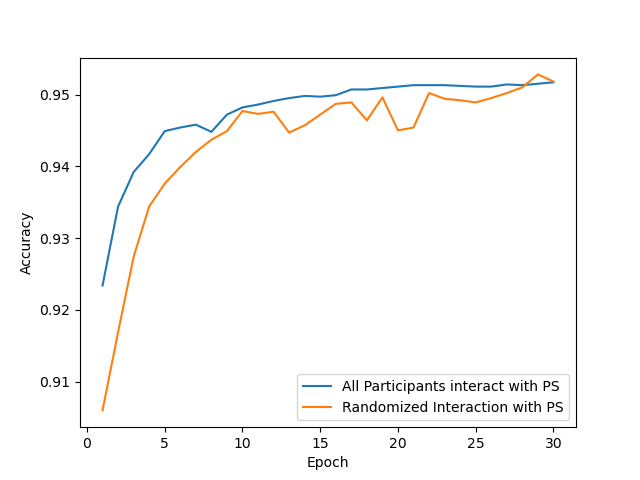
\includegraphics[width=8cm, keepaspectratio]{RandomVsAll}
\caption{Comparison between randomized interaction and complete interaction with server. }
\label{fig:RandVsAll}
\end{figure}

\begin{figure}[!h]
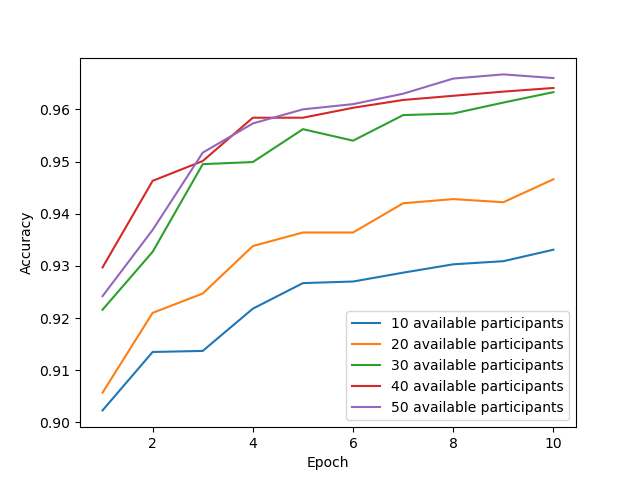
\includegraphics[width=8cm, keepaspectratio]{VaryingPoolofParticipants}
\caption{Accuracy of Distributed SGD for varying participants available for interaction with the PS.}
\label{fig:VaryingPoolofParticipants}
\end{figure}

\begin{figure}[!h]
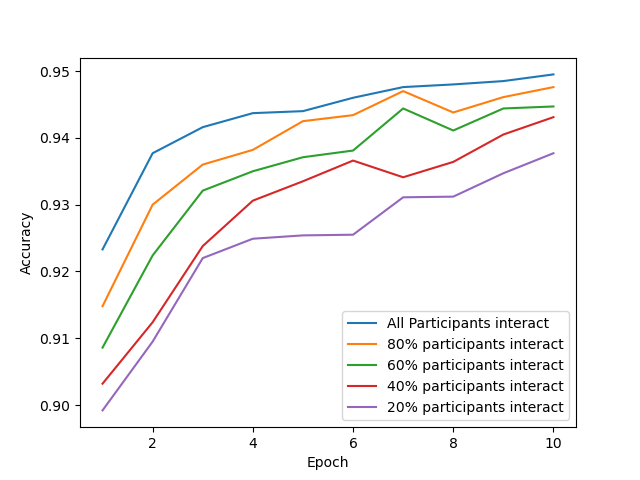
\includegraphics[width=8cm, keepaspectratio]{VaryingProbabilityInteraction}
\caption{Accuracy of Distributed SGD for varying proability of interaction with the PS. }
\label{fig:VaryingProbabilityInteraction}
\end{figure}


\begin{figure}[!h]
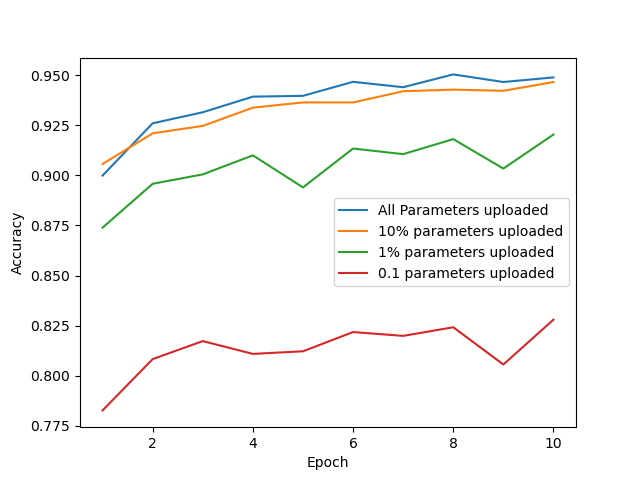
\includegraphics[width=8cm, keepaspectratio]{VaryingThetaU}
\caption{Accuracy of Distributed SGD for different upload gradient selection rate, unevenly. }
\label{fig:VaryingThetaU}
\end{figure}


\begin{figure}[!h]
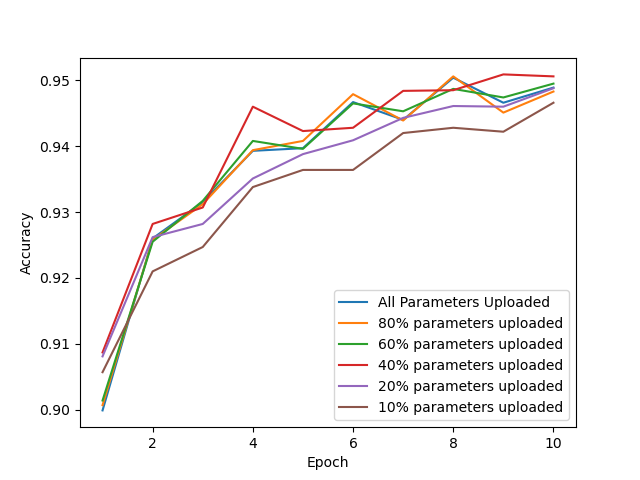
\includegraphics[width=8cm, keepaspectratio]{VaryingThetaUEvenly}
\caption{Accuracy of Distributed SGD for different upload gradient selection rate, Evenly. }
\label{fig:VaryingThetaUEvenly}
\end{figure}

\section{Conclusion}


\section{Authors and Affiliations}


\section{Identify the Headings}


\section{Figures and Tables}



\bibliographystyle{IEEEtran}
\bibliography{references}


\end{document}
